\section{Procedimentos Experimentais}
Esta seção descreve detalhadamente todos os procedimentos adotados na realização do experimento, de modo a permitir sua completa reprodutibilidade. As etapas foram divididas em duas partes: levantamento da curva característica do diodo (\textit{Procedimento 2a}) e análise das respostas dinâmicas do dispositivo em diversas configurações sob excitação senoidal (\textit{Procedimento 2b}).

\subsection{Procedimento 2a: Levantamento da Curva Característica $I_D \times V_D$ do diodo BY127.}

\hspace{1cm}Após a montagem do circuito (Figura~\ref{fig:CircA}), procedeu-se à variação da queda de tensão sobre o diodo ($V_D$) em incrementos de $100~mV$. Para cada incremento, foi registrada a respectiva corrente ($I_D$) que atravessava o componente. Estabeleceu-se um limite máximo de corrente de $40~mA$, visando preservar a integridade física do diodo.

\subsubsection{a) Polarização direta}

Inicialmente, foi montado um circuito composto por uma fonte de tensão contínua ajustável, um resistor de \(100~\Omega\) (\(\pm 5\%\)) e um diodo BY127 conectado em série. O objetivo era aplicar diferentes tensões ao diodo e medir a corrente resultante no circuito.

\begin{enumerate}
    \item Ajustou-se a fonte de tensão para o valor inicial de \(0{,}1~\mathrm{V}\).
    \item Mediu-se a corrente total do circuito utilizando um amperímetro digital conectado em série.
    \item Registrou-se também a tensão diretamente sobre o diodo por meio de um voltímetro digital conectado em paralelo ao componente.
    \item A tensão aplicada foi aumentada em incrementos de \(0{,}1~\mathrm{V}\), repetindo-se as medições para cada valor, até que a corrente atingisse aproximadamente \(40~\mathrm{mA}\).
    \item Todos os dados foram registrados para posterior construção da curva característica.
\end{enumerate}

Essa etapa permitiu a identificação da tensão limiar de condução e da região exponencial da curva característa.
\hspace{1cm}Para concluir esta etapa, os terminais da fonte de tensão foram invertidos, repetindo-se a metodologia para a condição de polarização reversa do diodo.

\begin{figure}[h]
    \centering
    \includegraphics[width=5cm]{imagens/figA.pdf}
    \caption{Circuito do procedimento A}
    \label{fig:CircA}
\end{figure}

\subsubsection{b) Polarização reversa}

Para determinar a característica do diodo em polarização reversa, o sentido do diodo na montagem anterior foi invertido.

\begin{enumerate}
    \item Com o diodo invertido, ajustou-se novamente a fonte DC para \(0{,}1~\mathrm{V}\).
    \item Mediu-se a corrente reversa utilizando o amperímetro em série.
    \item A tensão foi aumentada gradualmente, como na etapa anterior, observando-se o comportamento da corrente.
    \item Os valores foram anotados até o limite operacional, equivalente ao máximo permitido pela fonte de alimentação (aprox. $50~V$, muito abaixo da tensão máxima reversa, que é de $800~\mathrm{V}$).
\end{enumerate}

Esta etapa permitiu verificar a corrente de saturação reversa, bem como a ausência de condução significativa abaixo da tensão de ruptura.

%\noindent\textit{B. Análise de Circuitos com diodos BY127.}
\subsection{Procedimento 2b: Análise de Montagens sob Excitação Senoidal}

\hspace{1cm}Nesta etapa, realizou-se a montagem de cada circuito proposto na Figura~\ref{fig:CircB}. Em todas as configurações, a fonte de alimentação forneceu um sinal senoidal com amplitude de $8~V_{pp}$ (pico a pico) e frequência de $100~Hz$.

\hspace{1cm}Para cada montagem, foram registrados (fotografados) os sinais de entrada e de saída observados no osciloscópio. Foi dada especial atenção à mensuração da atenuação e da defasagem entre as respectivas formas de onda.

\vspace{-.5cm}

\begin{figure}[h]
    \centering
    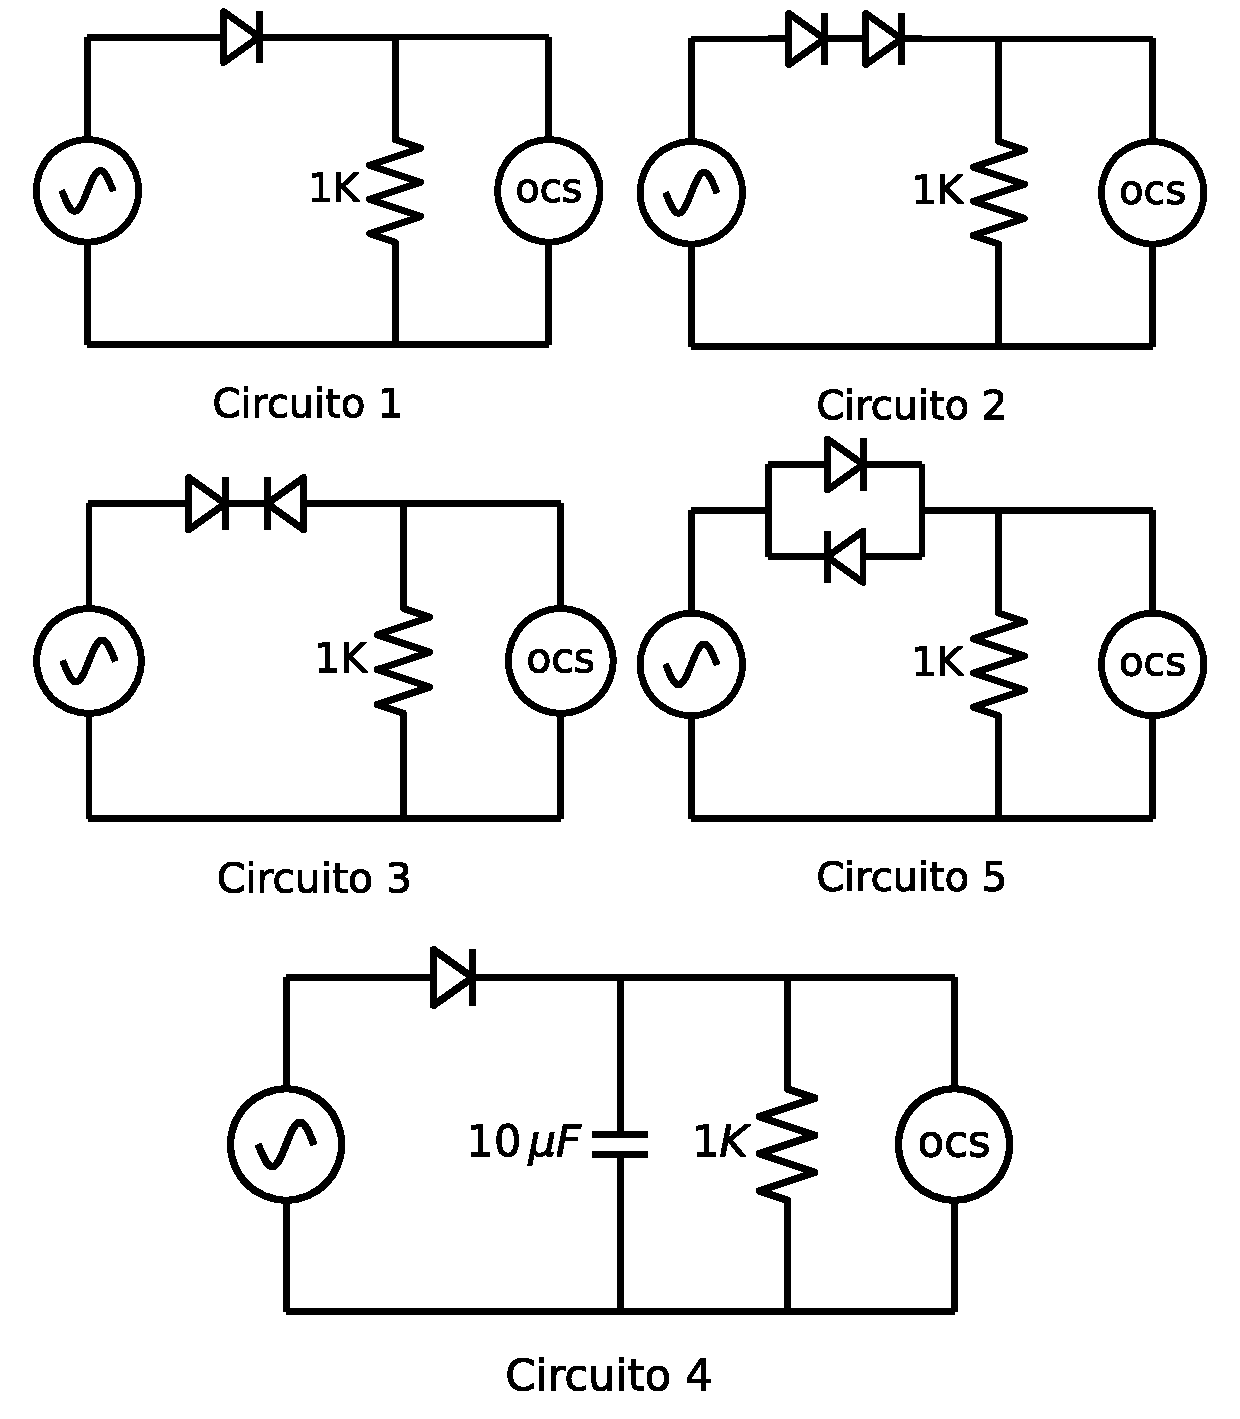
\includegraphics[width=7cm]{imagens/FigB.pdf}
    \caption{Circuitos do procedimento B}
    \label{fig:CircB}
\end{figure}

A segunda parte do experimento consistiu em analisar a resposta temporal de diferentes topologias de retificação utilizando o diodo BY127. Em todos os casos, aplicou-se ao circuito uma tensão senoidal de amplitude \(8~\mathrm{V_{pp}}\) e frequência \(100~\mathrm{Hz}\), proveniente de uma fonte CA ajustável.

A tensão observada no resistor de carga foi monitorada por meio de um osciloscópio digital, configurado para medir a forma de onda resultante da condução do diodo.

As montagens realizadas foram:

\begin{enumerate}
    \item \textbf{Um diodo em série com o resistor}: configuração clássica de retificação de meia onda.
    \item \textbf{Dois diodos em série}: aumento da queda direta total, modificando o limiar de condução.
    \item \textbf{Dois diodos em antissérie}: bloqueio mútuo dos semiciclos, resultando em condução mínima.
    \item \textbf{Dois diodos em antiparalelo}: cada diodo conduz em um semiciclo, permitindo passagem alternada.
    \item \textbf{Um diodo em série com um filtro capacitivo (capacitor em paralelo com o resistor)}: implementação de um retificador de meia onda com suavização da tensão.
\end{enumerate}

Para cada uma das cinco montagens, adotou-se o seguinte procedimento:

\begin{enumerate}
    \item Conectou-se o circuito correspondente na protoboard, verificando a polaridade dos diodos.
    \item Ajustou-se a fonte CA para fornecer \(8~\mathrm{V_{pp}}\) a \(100~\mathrm{Hz}\).
    \item Configurou-se o osciloscópio para registrar a tensão sobre o resistor de carga.
    \item Observou-se a forma de onda resultante, anotando suas características gerais, incluindo recortes, distorções, níveis de pico e presença de ripple (quando aplicável).
    \item Fotografou-se a tela do osciloscópio para posterior inclusão no relatório.
    \item Mediu-se o atraso de condução (\textit{delay}) associado a cada configuração. \\
\end{enumerate}

Esses procedimentos possibilitaram a análise comparativa entre o comportamento ideal e o comportamento real dos circuitos retificadores, fornecendo subsídios para a discussão apresentada na seção de resultados.
%\vspace{-.75cm}
